\chapter{\textbf{Конструкторский раздел}}

Цель данной работы -- определить, какой тип документа загрузил пользователь.

Классификатор получает входные данные: фотографию документа. На выходе классификатор сообщает, что он получил (паспорт, водительское удостоверение или какие-либо другие типы документов).

\section{Функциональная модель}

На рисунке \ref{img:idef0} изображен нулевой уровень декомпозиции задачи. 

\begin{figure}[H]
	\centering
	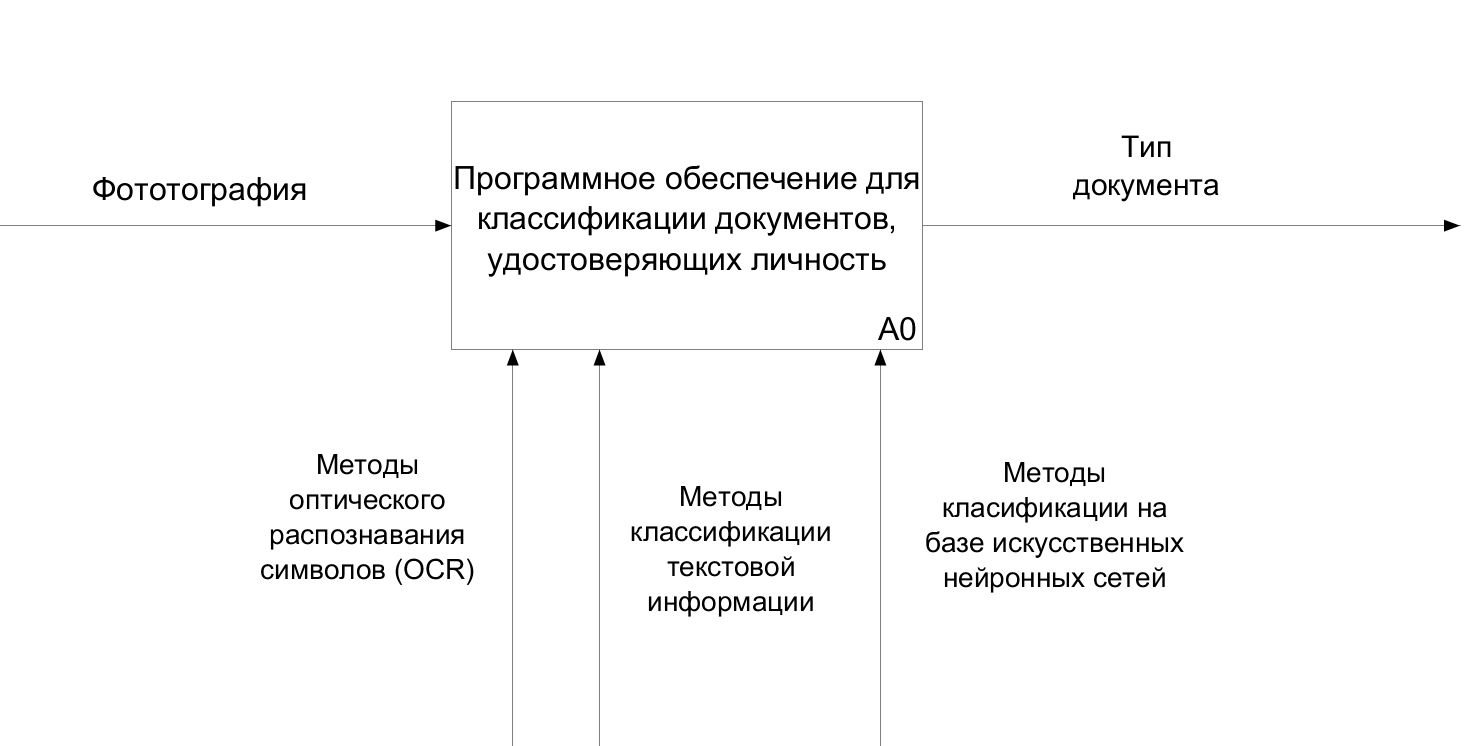
\includegraphics[scale=0.3]{idef0}
	\caption{Нулевой уровень декомпозиции задачи. }
	\label{img:idef0}
\end{figure}

На вход классификатору поступает изображение, которое после предобработки поступает на вход классификатора по визуальным признакам. Также изображение поступает на вход системе оптического распознавания символов и после предобработки, текст поступает на вход классификатора по текстовым признака.

В данной работе будет представлен алгоритм объединения двух классификаторов.

На основе выделенных этапов, был предложен подход к декомпозиции разрабатываемого метода, приведенный на рисунке \ref{img:idef01}.

\begin{figure}[H]
	\centering
	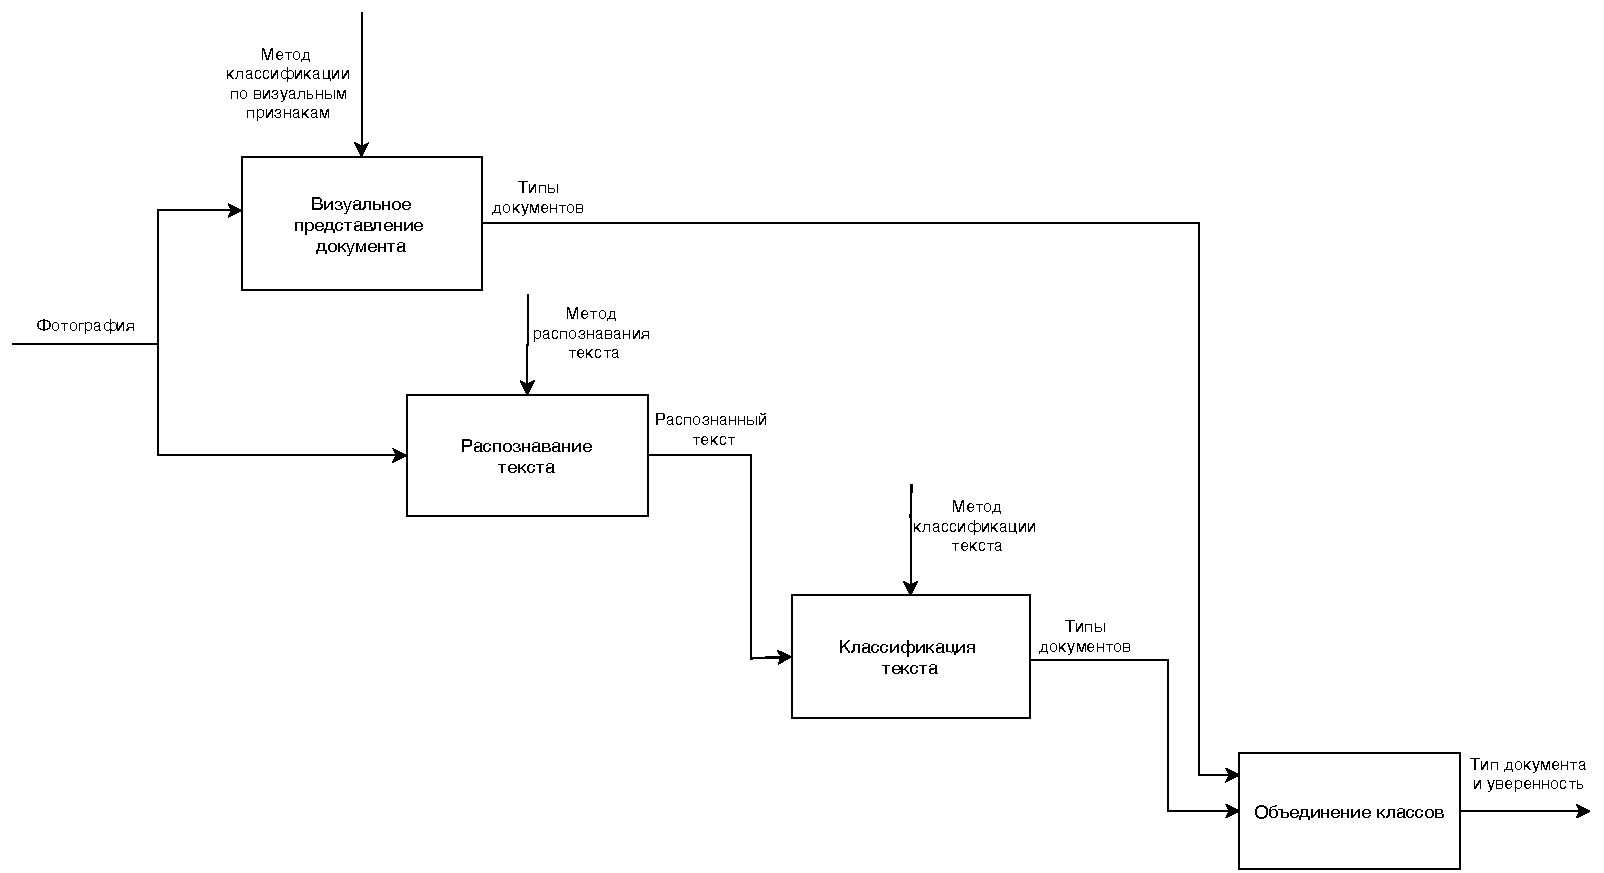
\includegraphics[scale=0.3]{idef01}
	\caption{Функциональная модель первого уровня. }
	\label{img:idef01}
\end{figure}

Далее необходимо рассмотреть каждый из этапов.

\section{Предобработка изображения и классификация по визуальным признакам}

Свёрточная нейронная сеть googlenet принимает изображения формата 224х224, поэтому изначально изображения нужно привести к исходному формату.

На рисунке \ref{img:googlenet} представлена модель данной нейронной сети.

Она состоит из следующих слоев.
\begin{itemize}
\item Сверточный слой -- применение операции свертки к выходам с предыдущего слоя, где веса ядра свертки являются обучаемыми параметрами. 
\item Пулинговый слой призван снижать размерность изображения. Исходное изображение делится на блоки размером $w \times h$ и для каждого блока вычисляется некоторая функция. В данной модели, в основном, используются функции максимума (max pooling) и среднего (average pooling). 
\item  Inception -- это специальный слой нейронной сети, впервые представленный в googlenet. Данный слой является небольшой локальной сетью и его задача состоит в параллельном применении нескольких фильтров на исходное изображение, которые затем объединяются в один выходной. Данный слой позволяет сохранить малое число слоев, с сохранением полезной информации о изображении.
\item  Двумя проблемами в обучении глубоких нейронных сетей являются исчезающий градиент и взрывающийся градиент. Для борьбы с этой проблемой был предложен слой исключения (residual block). Идея заключается в том, чтобы взять пару слоёв (например, свёрточных), и добавить дополнительную связь, которая проходит мимо этих слоёв. 
\item  Softmax -- функция, которая превращает вектор действительных чисел в вектор вероятностей. 
\end{itemize}

Все скрытые слои используют функцию активации ReLU.
 
\begin{figure}[H]
	\centering
	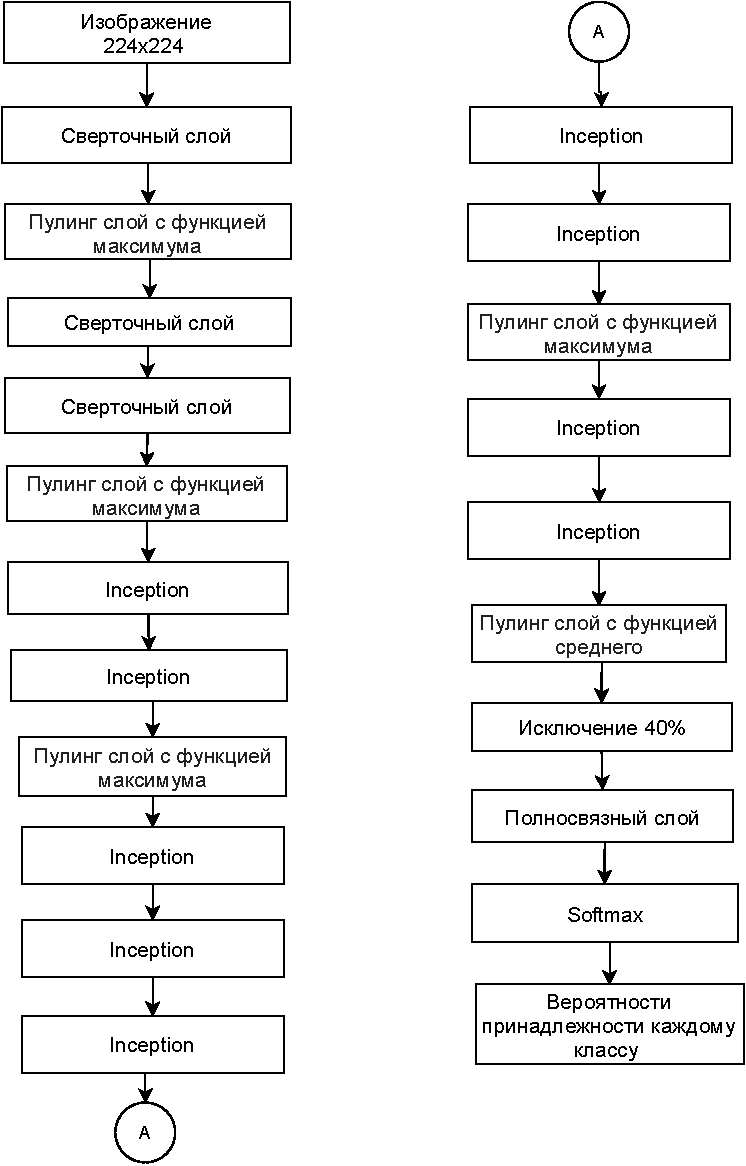
\includegraphics[scale=1]{googlenet}
	\caption{Схема модели нейронной сети googlenet. }
	\label{img:googlenet}
\end{figure}

На выходе получаем вероятности принадлежности документа к каждому из классов, необходимо выбрать максимальную.

Перед началом обучения необходимо определить размер выборки. Размер выборки обусловлен точностью определения параметров метода и необходимой сложностью исследования. Для оценки размера выборки можно воспользоваться законом больших чисел, записанном в форме 2-ого неравенства Чебышева \ref{eq:cheb}. \cite{cheb}

\begin{equation}
	\centering
	P = \{|X-MX| \geq \varepsilon\}\leq \frac{\sigma^2}{N\varepsilon^2}
	\label{eq:cheb}
\end{equation}

$N$ -- размер выборки.

$X$ -- случайная величина.

$\varepsilon$ -- требуемая точность.

$\sigma$ -- дисперсия случайной величины.

При достоверности метода $P= 0,9$, а точность $\varepsilon=0.05$, тогда $N=1000$.

Данная нейронная сеть обучалась на выборке в 800 фотографий, из них страницы паспорт РФ и загранпаспорт -- примерно по 120 изображений на каждый класс, водительские удостоверения -- по 60 на каждый класс, визы представлены самым меньшим количеством данных -- менее 30 на каждый класс.

\section{Извлечение текста из изображения, его предобработка и классификация}

Как говорилось ранее извлечение текста из изображения проходит с помощью методов оптического распознавания символов, а именно tesseract.

Для возможности дальнейшей классификации, текст необходимо предобработать.

\begin{itemize}
\item Во-первых, для уменьшения его объема (очистка от пунктуации и пустых строк).
\item Во-вторых, для улучшения точности значимости оценки слов, необходимо очистить текст от стоп-слов -- союзов, предлогов и прочего.
\item Также необходимо привести все слова к одному регистру, чтобы можно было сравнивать их.
\item После этого можем провести векторизацию текста для получения вектора слов и их весов.
\end{itemize}

Схема алгоритма предобработки текста представлена на рисунке \ref{img:preprocessing}.

\begin{figure}[H]
	\centering
	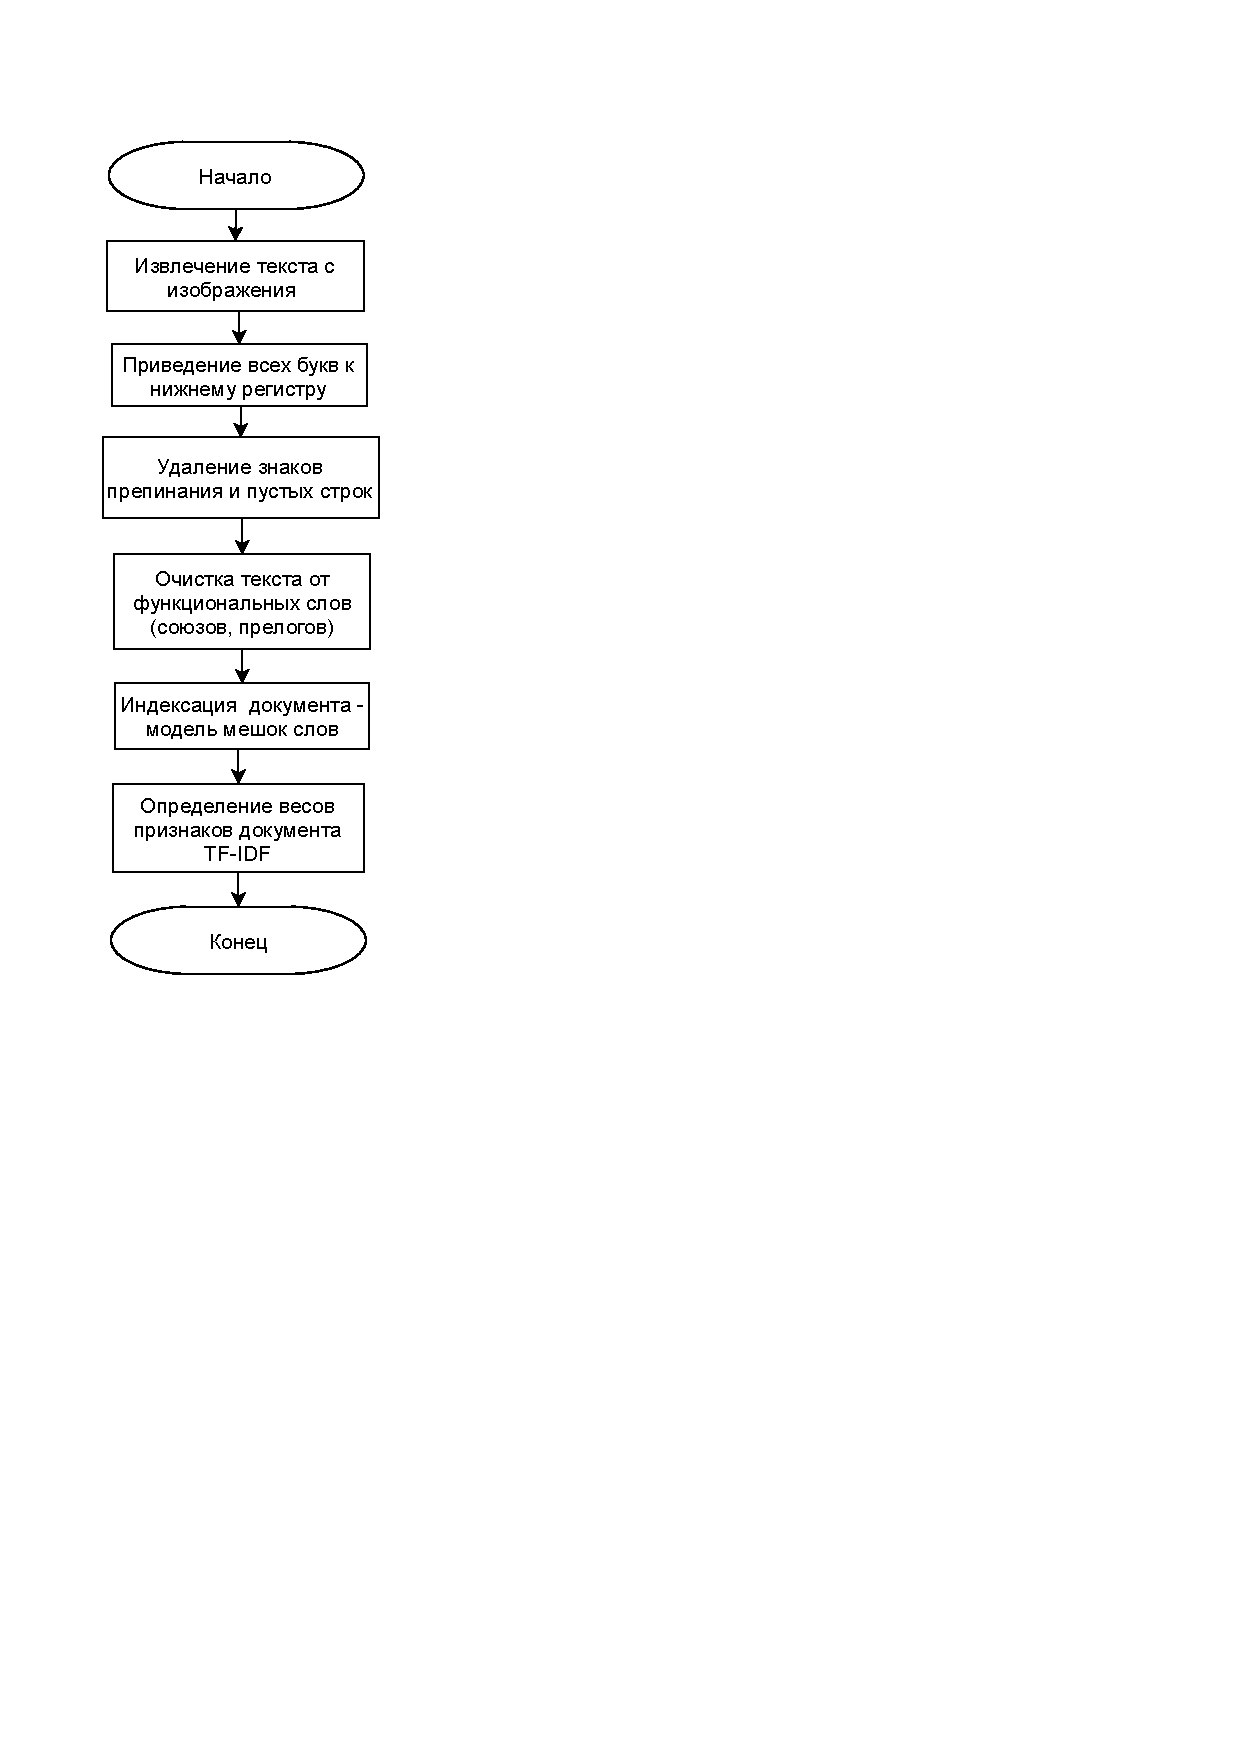
\includegraphics[scale=1.2]{preprocessing}
	\caption{Схема алгоритма предобработки текста. }
	\label{img:preprocessing}
\end{figure}

Таким образом, после выполнения данного этапа мы получаем векторное представление нашего текста.

Можно показать облако слов для классифицируемых в данной работе документов, представлено на рисунке \ref{img:cloudwords}. 

Облако слов или тегов -- это визуальное представление ключевых слов. 

\begin{figure}[H]
	\centering
	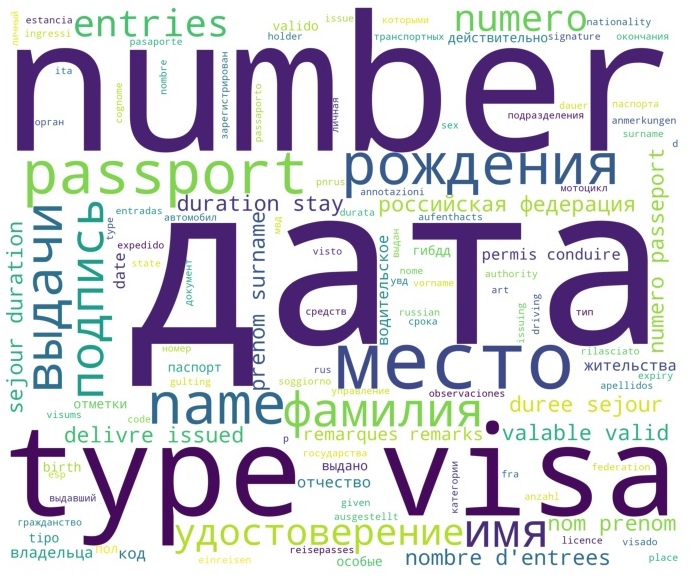
\includegraphics[scale=0.5]{cloudwords}
	\caption{Облако слов документов. }
	\label{img:cloudwords}
\end{figure}

После получения векторного представления нашего текста, можно классифицировать его методом опорных векторов. Обучающая выборка такая же, как и для googlenet.

\section{Объединение}

Следующий этап -- объединение результатов.

\textbf{Ансамбль методов} использует несколько обучающих алгоритмов с целью получения лучшей эффективности прогнозирования, чем могли бы получить от каждого обучающего алгоритма по отдельности.

Будет проходить с помощью взвешенного голосования.

Рассмотрим задачу, имеем 11 классов: $Y=\{1,2,...K\}, K=11$.

И 2 классификатора или эксперта: $f_1, ...f_M, M=2$.

Тогда результат голосования будет представлен формулой \ref{eq:voute}, где \ref{eq:ivoute} и $\alpha_i$ -- вес голоса i-ого эксперта.

\begin{equation}
	\centering
	f(x)=\max_{k=1..K}\sum_{i=1}^M\alpha_i I(f_i(x)=k), \sum_i \alpha_i=1, \alpha_i>0
	\label{eq:voute}
\end{equation}

\begin{equation}
	\centering
	I(x) = \begin{cases}
   1 &\text{x = true}\\
   0 &\text{x = false}
 \end{cases}
	\label{eq:ivoute}
\end{equation}

Задача исследовательского раздела состоит в проведении многомерной оптимизации Нелдера-Мида для определения оптимальных весовых коэффициентов для каждого класса.

\section{Выборка}

Выборка представляет собой набор фотографий документов, на каждом из которых документ занимает более 80\% площади документа и располагается правильно (угол поворота относительно любой оси координат меньше 15 градусов). Также документы на фотографиях выборки хорошо освещены, находятся в фокусе и несмазаны.

Пример фотографии из выборки приведен на рисунке \ref{img:dataset}.

\begin{figure}[H]
	\centering
	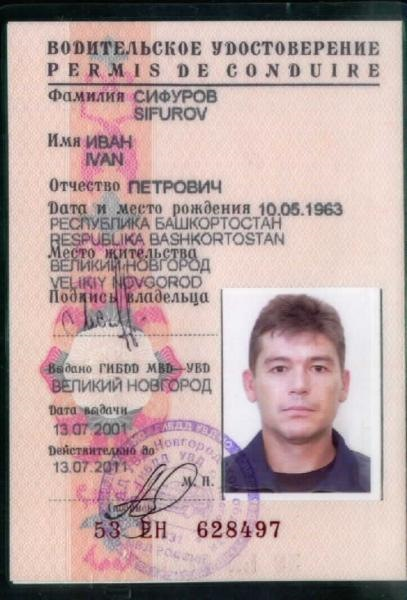
\includegraphics[scale=0.7]{dataset}
	\caption{Пример водительского удостоверения из выборки. }
	\label{img:dataset}
\end{figure}

\section{Вывод}

В данном разделе было проведено проектирование метода классификации документов, удостоверяющих личность, по фотографии.

Были описаны входные и выходные параметры каждого этапа. Так же была описана выборка данных, которая представляет собой набор фотографий. 

Для объединения двух классификаторов было решено использовать ансамбль классификаторов, использующих взвешенное голосование.